\section{Solution Design}
\label{sec:approach:solution}

Based on the definitions and constraints shown in Section \ref{sec:approach:def}, an offline system for extended activity model learning is presented. The objective of the system is to learn extended activity models (EAM, definition \ref{def-eam}) for every defined activity and a particular user, since every user has his/her own way to perform activities in terms of executed actions. The initial activity models (IAM, definition \ref{def-iam}) for every activity provided by a domain expert will be the same for every user, because they are generic models. But the extended activity models are personal models. They capture different complete activity models performed by a user. Notice that EAM learning has several implications in the ontology-based activity model approach:

\begin{enumerate}
 \item Complete models are learnt for every activity and a particular user. Complete refers to the sequence of executed actions for a concrete activity.
 \item If two or more different complete models are learnt for a concrete activity, specialised models of the same activity are found. This means that the defined activity is not a leaf in the ADL ontological tree and hence, sub-activities of that activity are discovered.
 \item Activity models can be dynamic. If the EAM learning system is continuously updated with new data, activity models can be updated. In consequence, activity models evolve and are adapted to users' varying behaviours.
\end{enumerate}

\subsection{Inputs of the learning system}
\label{subsec:approach:inputs}

The learning system for EAMs works on user generated data. It combines domain knowledge and user generated data in a learning algorithm. Notice that user data comes in an unlabelled sensor activation dataset, so there is no need to manually label any dataset. On the other hand, domain knowledge concerning the environment and activities is provided to the learning system. More concretely, the inputs of the EAM learning system are:

\begin{enumerate}
 \item Context knowledge: the context knowledge represents the prior knowledge provided by a domain expert which is relevant to learn activity models. The concepts modelled in the context knowledge include: 
 \begin{enumerate}
  \item Activities: every activity is defined by its name, type, location and IAM. Following definition \ref{def-type}, an activity has only one type. However, an activity can be performed in several locations (notice that this does not contradict constraint \ref{cons-location}). 
  \item Objects: objects refer to every object in the environment which is monitored by sensors and is used to perform activities. An object is defined by its name, type, location and attached sensors. As definition \ref{def-type} states, an object can have several types. But an object is subjected to constraint \ref{cons-static-obj}, so it has a unique location. In principle, objects can be monitored by several sensors. For instance, a fridge may have a tilt sensor attached to its door to monitor open/close door actions and an electric sensor to monitor the power usage.
  \item Sensors: following constraint \ref{cons-dense}, sensors are attached to objects and they are defined by a sensor identifier, type, described action and object to which is attached. Sensors produce sensor activations (definition \ref{def-sa}) when they transition from their no-interaction state to interaction state. Sensors have a unique type and they are mapped to one single action, as stated in definition \ref{def-action}. The object to which the sensor is attached is also stored in the context knowledge.
 \end{enumerate}
 
 \item Sensor activation dataset: as defined in definition \ref{def-sa-dataset}, an unlabelled timestamped sensor activation dataset with the activity traces of a concrete user.
\end{enumerate}

In the current implementation, context knowledge is formatted in a JavaScript Object Notation (JSON)\footnote{http://json.org/} file. JSON has been selected because it provides a light-weight knowledge formatting syntax which is widely supported and used to share information. Although OWL or RDF could be used to implement context knowledge, the overhead introduced by such markup languages comes without any advantage for the EAM learning system. The decision of using JSON responds to the principle of providing a simple solution, focusing on modelling only relevant knowledge. As an example, Figure \ref{fig-context-json} shows how an activity, an object and a sensor are modelled in the context knowledge file. This knowledge is provided by a domain expert and modelled by knowledge engineers. 

\begin{figure}[htbp]
\begin{small}
\begin{lstlisting}
"MakeCoffee": {
	"type": ["Cooking"],
	"location": ["Kitchen"],
	"IAM": ["hasContainer", "hasCoffee"],
	"duration": 300
}
---------------------------------------------------
"kitchen-tap": {
	"type": ["Cooking", "HouseWork"]
	"location": "Kitchen"
	"sensors": ["ktapSens"]
}
---------------------------------------------------
"ktapSens": {
	"type": "tilt",
	"action": "turnOnTap",
	"attached-to": "kitchen-tap"
}
\end{lstlisting}
\end{small}
\caption{Example of activities, objects and sensors modelled in the context knowledge file. Activity duration is given in seconds.}
\label{fig-context-json}
\end{figure}

The second input to the EAM learning system is the sensor activation dataset. For the implementation presented in this dissertation, sensor activation datasets are formatted in Comma Separated Value files (CSV)\footnote{http://en.wikipedia.org/wiki/Comma-separated\_values}. Each row of the file contains a timestamp (year, month, day and time) and a sensor activation tagged with the sensor identifier which has produced the activation (see Figure \ref{fig-dataset}).


\begin{figure}[htbp]
\begin{small}
\begin{lstlisting}
2014-05-23 09:47:33.984341,storeSens
2014-05-23 09:47:39.333528,potSens
2014-05-23 09:47:52.750216,cookerSens
2014-05-23 09:48:07.764138,fridgeSens
2014-05-23 09:48:12.591836,wmilkSens
2014-05-23 09:48:47.199512,chocoSens
2014-05-23 09:54:11.553695,mugSens
2014-05-23 09:54:40.794979,rcontrolSens
2014-05-23 09:54:50.390696,tvSens
2014-05-23 09:54:59.348862,sofaSens
\end{lstlisting}
\end{small}
\caption{A slice of a sensor activation dataset.}
\label{fig-dataset}
\end{figure}

Based on those inputs, a context knowledge file and a sensor activation dataset, the output of the EAM learning system is a list of action sequences for each activity, which describe the EAMs for each activity (see equation \ref{eq-eam}). 

\subsection{Intuition behind the solution}
\label{subsec:approach:intuition}
The rationale for the designed solution to EAM learning comes when sensor activations are plotted in a three-dimensional space spanned by location, type and time, as shown in Figure \ref{fig-action-plot}. This three-dimensional space, named activity space, reflects the prior knowledge about activities. An activity has a concrete type that is shared with the object types used to perform that activity and is performed in a location and a time segment. 

\begin{figure}[htbp]
\centering
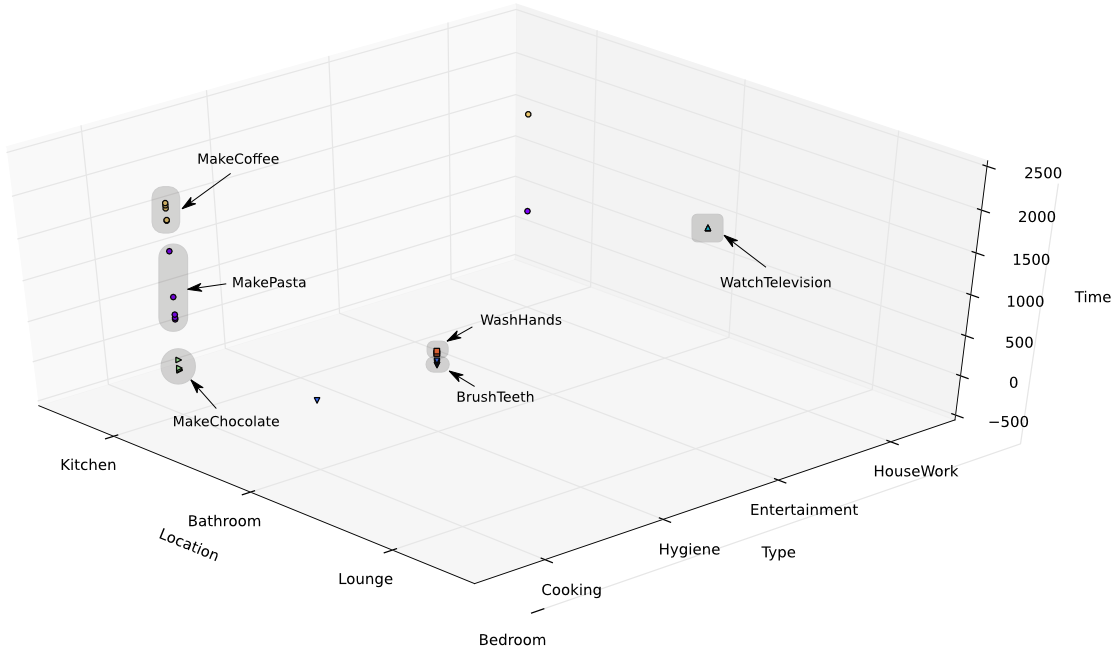
\includegraphics[width=\textwidth]{activity_visualization_m.png}
    \caption{A plot of the actions executed by a user for performing several activities in the three-dimensional space spanned by location, type and time.}
    \label{fig-action-plot}
\end{figure}

When sensor activations describing several activities are plotted in the activity space, several lumps or clusters can be distinguished. Intuition says that sensor activations, and hence actions, have to be close to each other when they form an activity (close in the activity space), i.e. if a user is making pasta, it is common sense to think that sensor activations describing that activity will be located in the kitchen, and the objects which are being used by the user will be for cooking purposes. As far as time regards, sensor activations will occupy a time segment which will denote the duration of the activity.

This grouping of actions in the activity space can be seen in Figure \ref{fig-action-plot}. Six activities can be identified there, namely MakeChocolate, BrushTeeth, WashHands, MakePasta, MakeCoffee and WatchTelevision. Due to time resolution in the graphic, actions composing BrushTeeth, WashHands and WatchTelevision cannot be properly distinguished. Those three activities are quite short in time, but depicted actions for each of them are respectively five, three and three. There are some actions that are not grouped in any activity. Those actions are generated by objects that have multiple types. For example, in the case of MakePasta, the kitchen tap is used. The kitchen tap can be used for cooking or for housework and that is why it appears in both positions.

It is interesting to see how Figure \ref{fig-action-plot} supports the intuition about action distribution in the activity space. In general, actions can be easily grouped in activities, but there are also some tough cases. This is the case of actions composing activities BrushTeeth and WashHands, which are very close in time and are performed in the same location and with the same purpose. The last action of MakePasta seems also difficult to group, since it is closer in time to activity MakeCoffee, sharing again the same location and type. 

In consequence, the idea is to design a clustering algorithm which takes advantage of location, type and time information to aggregate actions to clusters. The clustering process needs heuristics and metrics that take special care of those actions that are difficult to group in the corresponding activity. But this is not enough. Action clusters have to be identified and labelled with one of the defined activities. To identify action clusters with activity names, initial activity models in the context knowledge can be used. Initial activity models contain an incomplete sequence of actions. Despite being incomplete sequences, they can be used to identify activities. So the clustering algorithm has to produce several labelled action/sensor activation sequences per activity.

The clusters extracted in the clustering process may contain all the actions executed by a user to perform a concrete activity. Those clusters may be used to learn different ways of performing an activity and hence, to learn extended activity models. In summary, the key idea is to design a clustering algorithm that uses initial activity models to detect activities and some metrics in the activity space to aggregate actions to activities. Afterwards, using the clusters extracted and labelled, they are analysed to learn extended activity models for each activity.

%To learn those models a two-step system is presented. First, a clustering process is run in the so called \textbf{semantic space of actions}, using initial activity models to label each cluster with a modeled activity. The semantic space of actions is a three-dimensional space spanned by the axes of location, type and time. Actions carried out by a user have only one location in the environment (bathroom, kitchen etc.), one time instant, but multiple types. For instance, a glass can be used for multiple activity types, such as cooking, eating or personal hygiene (brushing teeth). Hence, the action \textit{hasContainer} linked to a glass activation, occupies multiple positions in the type axis. 

\subsection{Description of the solution}
Following the rationale described in section \ref{subsec:approach:intuition}, a solution for the EAM learning system has been designed. The devised system architecture is depicted in Figure \ref{fig-design}. At a first glance, the two important blocks identified in section \ref{subsec:approach:intuition} can be distinguished in the architecture: a clustering process and an activity model learning process. The clustering process is implemented in two modules, namely the Semantic Activity Annotation module ($SA^3$) and the Action Aggregator module ($AA$). On the other hand, the activity learning process is implemented by a module called Activity Model Learner ($AML$). 

\begin{figure}[htbp]
\centering
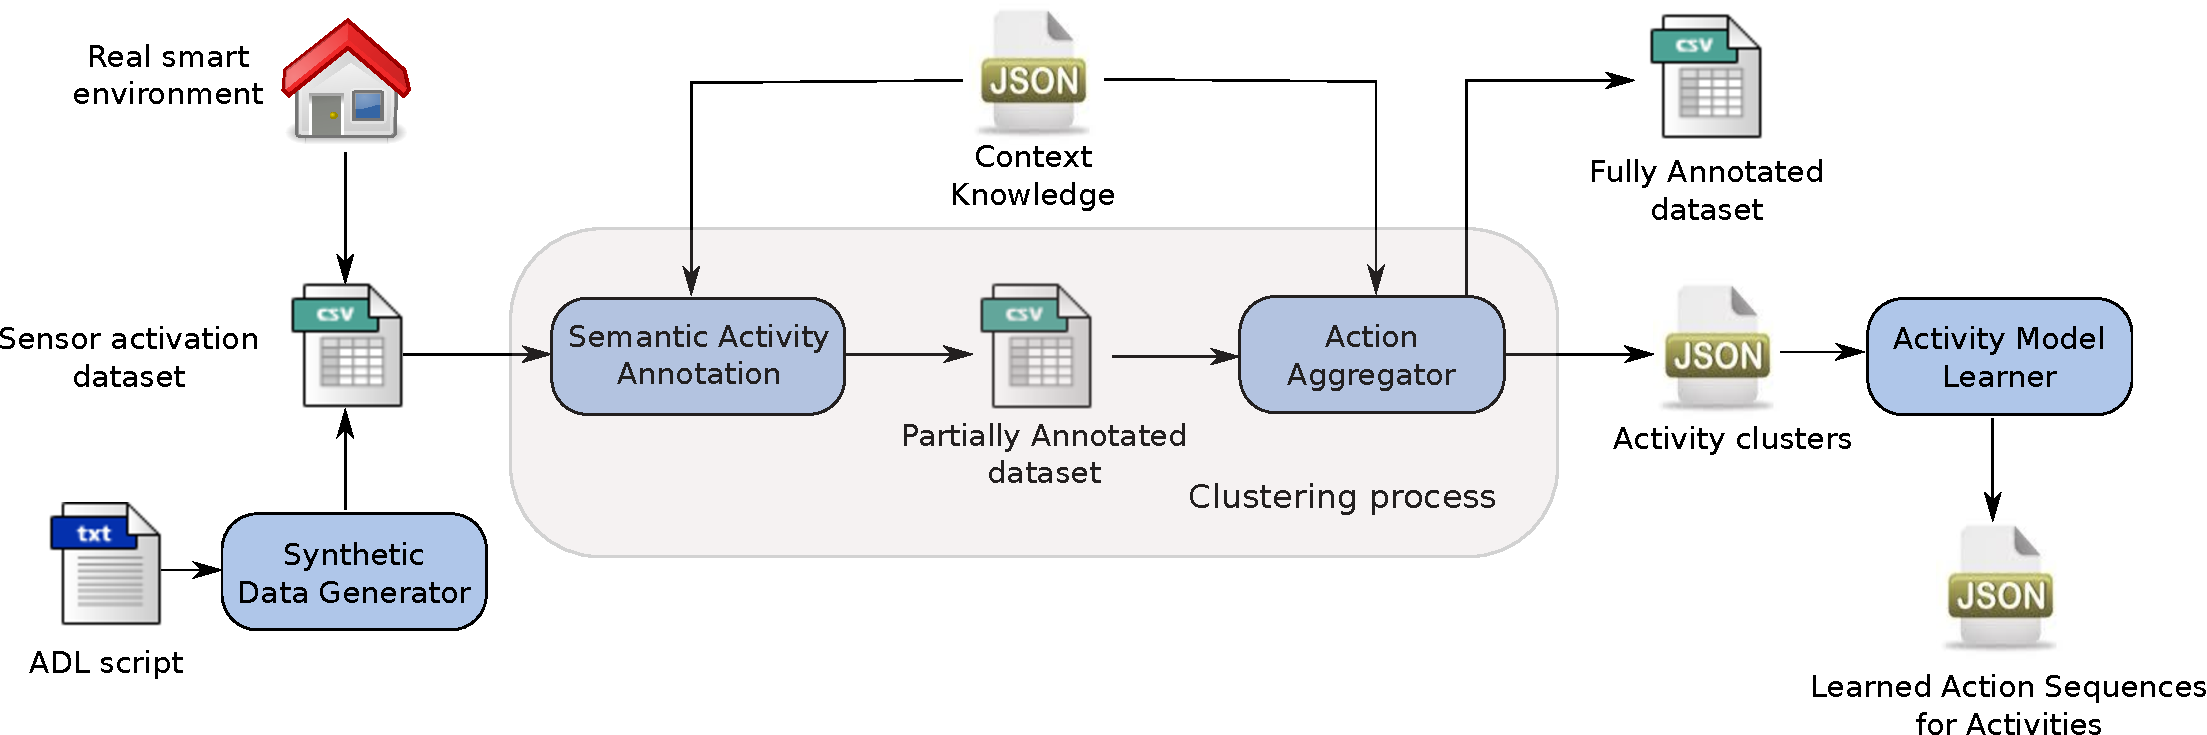
\includegraphics[width=\textwidth]{our_approach.pdf}
    \caption{The detailed design architecture of the proposed approach to learn EAMs.}
    \label{fig-design}
\end{figure}

Two kinds of elements can be distinguished in the architecture depicted in Figure \ref{fig-design}: files and software modules. The only exception to this rule is the \textit{real smart environment}, which represents a sensorised environment where a user performs several activities. All the other elements can be classified into files or software modules. There are three kinds of files: plain text files (\textit{ADL script}), JSON files (\textit{context knowledge}, \textit{activity clusters} and \textit{learnt action sequences for activities}) and CSV files (\textit{sensor activation dataset}, \textit{partially annotated dataset} and \textit{fully annotated dataset}). Files are used to exchange information between software modules. The developed software modules are four: \textit{Synthetic Data Generator}, \textit{Semantic Activity Annotation}, \textit{Action Aggregator} and \textit{Activity Model Learner}. All the software modules of the diagram have been implemented using Python 2.7\footnote{https://www.python.org/} and its packages Numpy\footnote{http://www.numpy.org/} for numerical computing and Pandas\footnote{http://pandas.pydata.org/} for data analysis. 

Once the elements of the architecture have been described, the solution itself will be detailed. Firstly, a sensor activation dataset has to be collected for a concrete user. A real smart environment or a synthetic data generator can be used to get this dataset. The sensor activation dataset contains all sensor activations registered for a user performing certain activities during a fixed period of time. Remember that sensor activations are unlabelled. Whatever method has been chosen to obtain it, the resulting sensor activation dataset is formatted in a CSV file and its information has already been described in definition \ref{def-sa-dataset}.

Afterwards, a novel clustering process is run on the sensor activation dataset, using the context knowledge provided by an expert and formatted in a JSON file. The proposed clustering process, which is extensively discussed in Chapter \ref{cha:clustering}, is divided into two steps: 

\begin{enumerate}
 \item Semantic Activity Annotation algorithm ($SA^3$): this algorithm uses IAMs stored in the context knowledge to detect activities in the unlabelled dataset. It transforms sensor activations to actions according to the given context knowledge to apply a novel pattern recognition algorithm that has been designed and implemented to detect the occurrence of IAMs in the unlabelled sensor activation dataset. $SA^3$ also uses object and activity location information to infer from sensor activations where an activity is being performed and analyse consequently the feasibility of the detected pattern. $SA^3$ is an initialisation process from the clustering point of view, because it finds initial clusters in the time axis and identifies the label of those clusters. The output of $SA^3$ is given in the so called \textit{partially annotated dataset}, where sensor activations and their resultant actions are labelled with activity names or the special label 'None', which indicates that the action could not be labelled with any known activity name. Notice that $SA^3$ only labels those actions that pertain to IAMs thus leaving the vast majority of actions without any label. This is the reason why the output of the algorithm is called \textit{partially annotated}. A detailed description of $SA^3$ is given in Section \ref{sec:clustering:sa3}.
 \item Action Aggregator algorithm ($AA$): the input to the algorithm is the output of $SA^3$, i.e. the partially annotated dataset file. $AA$ uses activity, object and action knowledge described in the context knowledge to expand initial action clusters detected by $SA^3$. To analyse those actions that remain unlabelled after $SA^3$, $AA$ defines boolean functions based on location, type and time information of actions and objects. It analyses unlabelled actions that are close to initial clusters, checking the feasibility of those actions pertaining to those close initial clusters. The feasibility is computed using location, type and time information, implementing the idea that actions pertaining to an activity are performed in the same location, with a coherent purpose and close in time. The $AA$ algorithm's result is stored in another CSV file called \textit{fully annotated dataset}, which assigns an activity label to all actions and their original sensor activations. The special label 'None' is used for those actions that are not considered part of any activity. Those actions can be originated by sensor noise or user erratic behaviour, i.e. a user that interacts with an object that is not being used for performing an activity. Additionally, $AA$ also generates a JSON file called \textit{activity clusters}. This file contains all the clusters found by the algorithm for each activity. Clusters, which are action sequences, come with an occurrence frequency. The activity clusters file is also used to store some interesting statistics found by $AA$ about the frequency of objects used and actions executed for each activity, frequency of locations where each activity has been performed and activity duration statistics (mean and standard deviation). An example of an activity clusters file can be seen in Figure \ref{fig-clusters-file}. The $AA$ algorithm is described in Section \ref{sec:clustering:ac}.
\end{enumerate}

\begin{figure}[htbp]
\begin{small}
\begin{lstlisting}
    "ReadBook": {
        "locations": [
            [42, "Bedroom"], 
            [11, "Lounge"]
        ], 
        "actions": [
            [53, "useFurniture"], 
            [53, "turnOnLamp"], 
            [53, "hasBook"]
        ], 
        "patterns": [
            [
                53, 
                [
                    "useFurniture", 
                    "turnOnLamp", 
                    "hasBook"
                ]
            ]
        ], 
        "objects": [
            [42, "bed"], 
            [42, "bedroom-lamp"], 
            [42, "book-b"], 
            [11, "sofa"], 
            [11, "lounge-lamp"], 
            [11, "book-a"]
        ], 
        "occurrences": 53, 
        "duration": [
            14.773584905660377, 
            2.6467602797835856
        ]
    }, 
\end{lstlisting}
\end{small}
\caption{Information stored in the activity clusters file for activity ReadBook.}
\label{fig-clusters-file}
\end{figure}

The main result of the clustering process is thus stored in the activity clusters JSON file. This file has the information of all action sequences executed by a user to perform a concrete activity. For example, in the file shown in Figure \ref{fig-clusters-file}, in the ``patterns'' section, all the action sequences found by $AA$ are stored. In this case, for activity ReadBook, only one cluster has been generated with 53 occurrences in the sensor activation dataset. According to $AA$, ReadBook has been performed by means of executing the action sequence \textit{useFurniture}, \textit{turnOnLamp} and \textit{hasBook}. Nevertheless, $AA$ generally finds many different clusters per activity. Those clusters are finally processed by Activity Model Learner ($AML$), which filters incorrect action sequences and outliers to learn final EAMs as a list of action sequences. $AML$ uses action sequence similarity metrics to implement an outlier detection algorithm. Notice that all action sequences or clusters detected by $AA$ are not valid activity models, since they may contain incorrectly labelled actions (due to clustering errors, sensor errors and/or user erratic behaviour) and missed actions (due to sensor errors). Those spurious action sequences have to be detected and removed, to discover those action sequences that are valid models for a given activity. Valid action sequences are the EAMs for activities and are stored in a JSON file called \textit{learnt action sequences for activities}. All the details about $AML$ are provided in Chapter \ref{cha:learner}.